\section{Technical Overview}
\subsection{PIOP for cyclotomic ring arithmetic}
\label{sec:tech-overview-ring}

We give an overview of our PIOP for proving matrix-vector products $As = t$ over the cyclotomic ring $\ring_p = \ZZ_p[X]/(X^n+1)$, where $n = 2^\nu$ and $p \equiv 1 \pmod{2n}$. This is the $\ring$-algebraic core of lattice-based cryptography including MLWE/RLWE encryption, Dilithium/Falcon/Hawk signatures, FHE operation proofs, and Ajtai hash commitments. The full protocol is given in~\cref{sec:matrix-vector-pior}.

\paragraph{A CRT-domain sumcheck for ring arithmetic.}
Our starting observation is that since we target fully splitting rings, we can use the CRT isomorphism $\ring_p \cong \field_p^n$ to reduce ring multiplication to pointwise multiplication. If $C \in \field_p^{n \times n}$ denotes the CRT matrix with entries $C_{k,\ell} = \omega^{(2k+1)\ell}$ (where $\omega$ is a primitive $2n$-th root of unity), then $As = t$ in $\ring_p^N$ is equivalent to the pointwise identity
\begin{equation}\label{eq:overview-pointwise}
    t_C(i,k) = \sum_{j=0}^{M-1} A_C(i,j,k) \cdot s_C(j,k) \qquad \text{for all } (i,k) \in [N] \times [n],
\end{equation}
where $A_C = C A$, $s_C = Cs$, and $t_C = Ct$ denote the CRT transforms applied to coefficient vectors.

As in the main construction, we never materialize these CRT transforms as committed polynomials. Instead, from the coefficient-domain multilinear extensions $\tilde{A}$, $\tilde{s}$, $\tilde{t}$ and the CRT-matrix multilinear extension $\tilde{C}$, we define the virtual polynomials
\[
    A_C(i,j,k) := \sum_{\ell \in \bits^\nu} \tilde{C}(k,\ell) \cdot \tilde{A}(i,j,\ell), \qquad
    s_C(j,k) := \sum_{\ell \in \bits^\nu} \tilde{C}(k,\ell) \cdot \tilde{s}(j,\ell), \qquad
    t_C(i,k) := \sum_{\ell \in \bits^\nu} \tilde{C}(k,\ell) \cdot \tilde{t}(i,\ell).
\]
On Boolean inputs, these agree with the actual CRT-domain values by linearity. 

The protocol instance includes oracles for $\tilde{A}$, $\tilde{s}$, $\tilde{t}$ (you may think of these as either prover or indexer-provided, depending on the setting). The verifier moves first, sampling $\alpha \in \extensionfield^\tau$ and $\alpha' \in \extensionfield^\nu$, and the prover sends $e_t$ claimed to equal $t_C(\alpha,\alpha')$. Next sumcheck is run on
\[
    e_t = \sum_{(j,k) \in \bits^{\mu+\nu}} A_C(\alpha, j, k) \cdot s_C(j, k) \cdot \meq(k, \alpha').
\]
This is a $(\mu+\nu)$-round sumcheck: the $\bm{J}$-rounds are degree~$2$, while the $\bm{K}$-rounds are degree~$3$. At the end, the verifier has random challenges $(\beta,\gamma) \in \extensionfield^{\mu+\nu}$ and a reduced claim $\sigma' = A_C(\alpha,\beta,\gamma) \cdot s_C(\beta,\gamma) \cdot \meq(\gamma,\alpha')$. The prover then sends explicit claims $e_A = A_C(\alpha,\beta,\gamma)$ and $e_s = s_C(\beta,\gamma)$, and the verifier checks $\sigma' = e_A \cdot e_s \cdot \meq(\gamma,\alpha')$.

To connect the virtual CRT-domain claims back to the committed coefficient-domain oracles, the verifier samples a batching challenge $\xi \in \extensionfield$ and the parties run another $\nu$ round sumcheck on the claim
\[
    e_A + \xi \cdot e_s + \xi^{2} \cdot e_t
    = \sum_{\ell \in \bits^{\nu}} \Big[\tilde{C}(\gamma, \ell) \cdot \big(\tilde{A}(\alpha, \beta, \ell) + \xi \cdot \tilde{s}(\beta, \ell)\big) + \xi^{2} \cdot \tilde{C}(\alpha', \ell) \cdot \tilde{t}(\alpha, \ell)\Big].
\]
Notice that $A_C$ and $s_C$ are opened at the CRT point $\gamma$ produced by the first sumcheck, while $t_C$ remains tied to the original point $\alpha'$. After the verifier samples a final challenge $\delta \in \extensionfield^\nu$, the protocol reduces to three ordinary evaluation claims on $\tilde{A}$, $\tilde{s}$, and $\tilde{t}$, together with two evaluation claims $\tilde{C}(\gamma,\delta)$ and $\tilde{C}(\alpha',\delta)$ which we show can be computed in $O(n)$ time (\cref{lem:m-eval}).

\paragraph{Holographic variant and reduced sumcheck.}
When $A$ is public, the indexer can supply the CRT-domain oracle $A_C$ directly. If in addition the claimed value $e_t = t_C(\alpha,\alpha')$ is public or the claimed evaluation of a virtual polynomial, then the only remaining committed CRT-consistency obligation is for $\tilde{s}$. In that case, we can inline the CRT expansion of $s_C$ directly into the first sumcheck and eliminate the second sumcheck entirely:
\[
    e_t = \sum_{(j,\ell) \in \bits^{\mu+\nu}} A_C(\alpha, j, \alpha') \cdot \tilde{C}(\alpha', \ell) \cdot \tilde{s}(j, \ell).
\]
This merged sumcheck has degree~$2$ in every round, saves $3\nu + 2$ field elements and $\nu+1$ rounds relative to the base protocol, and leaves only a single evaluation claim on the committed oracle $\tilde{s}$.

\paragraph{Ring Plonkish SNARK example.}
\label{sec:tech-overview-speedyspartan}
We informally sketch how our PIOR can yield a SNARK for ring Plonkish, building on SpeedySpartan. The highly optimized final variant we arrive at reflects the strength and composability of our protocol design as well as the PIOR framework.

\paragraph{Security.}
We prove round-by-round knowledge soundness by decomposing the protocol into PIOR building blocks and bounding the knowledge error of each. This modular viewpoint makes the ring-arithmetic subprotocol compose cleanly with other RBRKS arguments. Applying Fiat--Shamir to the resulting public-coin protocol then yields a non-interactive argument with the usual QROM knowledge guarantees.

\paragraph{Odd-prime tower fields.}
The core ring-arithmetic PIOP only requires a sufficiently large extension field $\extensionfield/\field_p$. The odd-prime tower from~\cref{sec:odd-prime-tower} is needed specifically for the DP25 ring-switch packing step in the oracle-reduction pipeline: it realizes the quadratic tower $\field_p \subset \field_{p^2} \subset \cdots \subset \extensionfield$ over an odd prime base field, so the packing reduction can run natively without changing the underlying arithmetization field.

\subsection{Polynomial commitment scheme implementation}
\subsection{sec:microlotus}
We implement \textit{microlotus}, a multilinear polynomial commitment scheme that combines the Basefold IOPP, random linear codes, our tower field construction for odd primes, ring-switch packing, and oracle skipping. Microlotus supports evaluating $v$-variate polynomials $f \in \field^{\multilin}[\vec{X}]$, for $\mathrm{char}(\field)>2$, at points $\vec{x} \in \extensionfield^v$ for any extension field $\extensionfield/\field$ such that $[\extensionfield:\field]$ is a power of two.

In the context of arithmetization, the choice of base field is driven primarily by the computation being arithmetized. The arithmetization overhead from a mismatched base field will almost always dominate the efficiency gains between being able to use one PCS versus another, so in this sense Microlotus is not directly comparable with schemes that don't support odd prime towers. With this caveat, we compare the performance of Microlotus against other schemes (Basefold, WHIR, Brakedown). Microlotus is instantiated over the degree 16 odd prime tower extension $\mathbb{K}$ of $\mathbb{F} = \mathbb{F}_{257}$, which corresponds to SWIFFT\footnote{In practice one should instead reparametrize SWIFFT around the modulus that works best for the rest of the circuit.}. Basefold below, refers to Basefold with Reed-Solomon using code rate $\frac{1}{2}$ and $100$ queries. Our benchmarks for WHIR are over a degree 3 Goldilocks extension. For Brakedown, they are over 
a $255$ bit prime field. We also compare our Basefold implementation over degree 3 Goldilocks for a fair comparison with WHIR. The following observations can be observed from our benchmarks of concrete performance:
\begin{itemize}
      \item The Microlotus prover is over 10x faster than WHIR and Basefold in prover time, and comparable to Brakedown for polynomial sizes of interest.
      \item The Microlotus verifier is over 10x faster than Brakedown and 2x faster than Basefold for larger polynomials, while still being about 6x slower than WHIR.
      \item Our proof size is a little less than twice as big as Basefold and WHIR, while being significantly smaller than Brakedown (the only scheme with square root proof size).
\end{itemize}
The benchmarks presented in this section were run \textit{single-threaded} on an AWS r7iz.8xlarge EC2 instance with 256 GB RAM.


\begin{figure}[t]
  \centering
  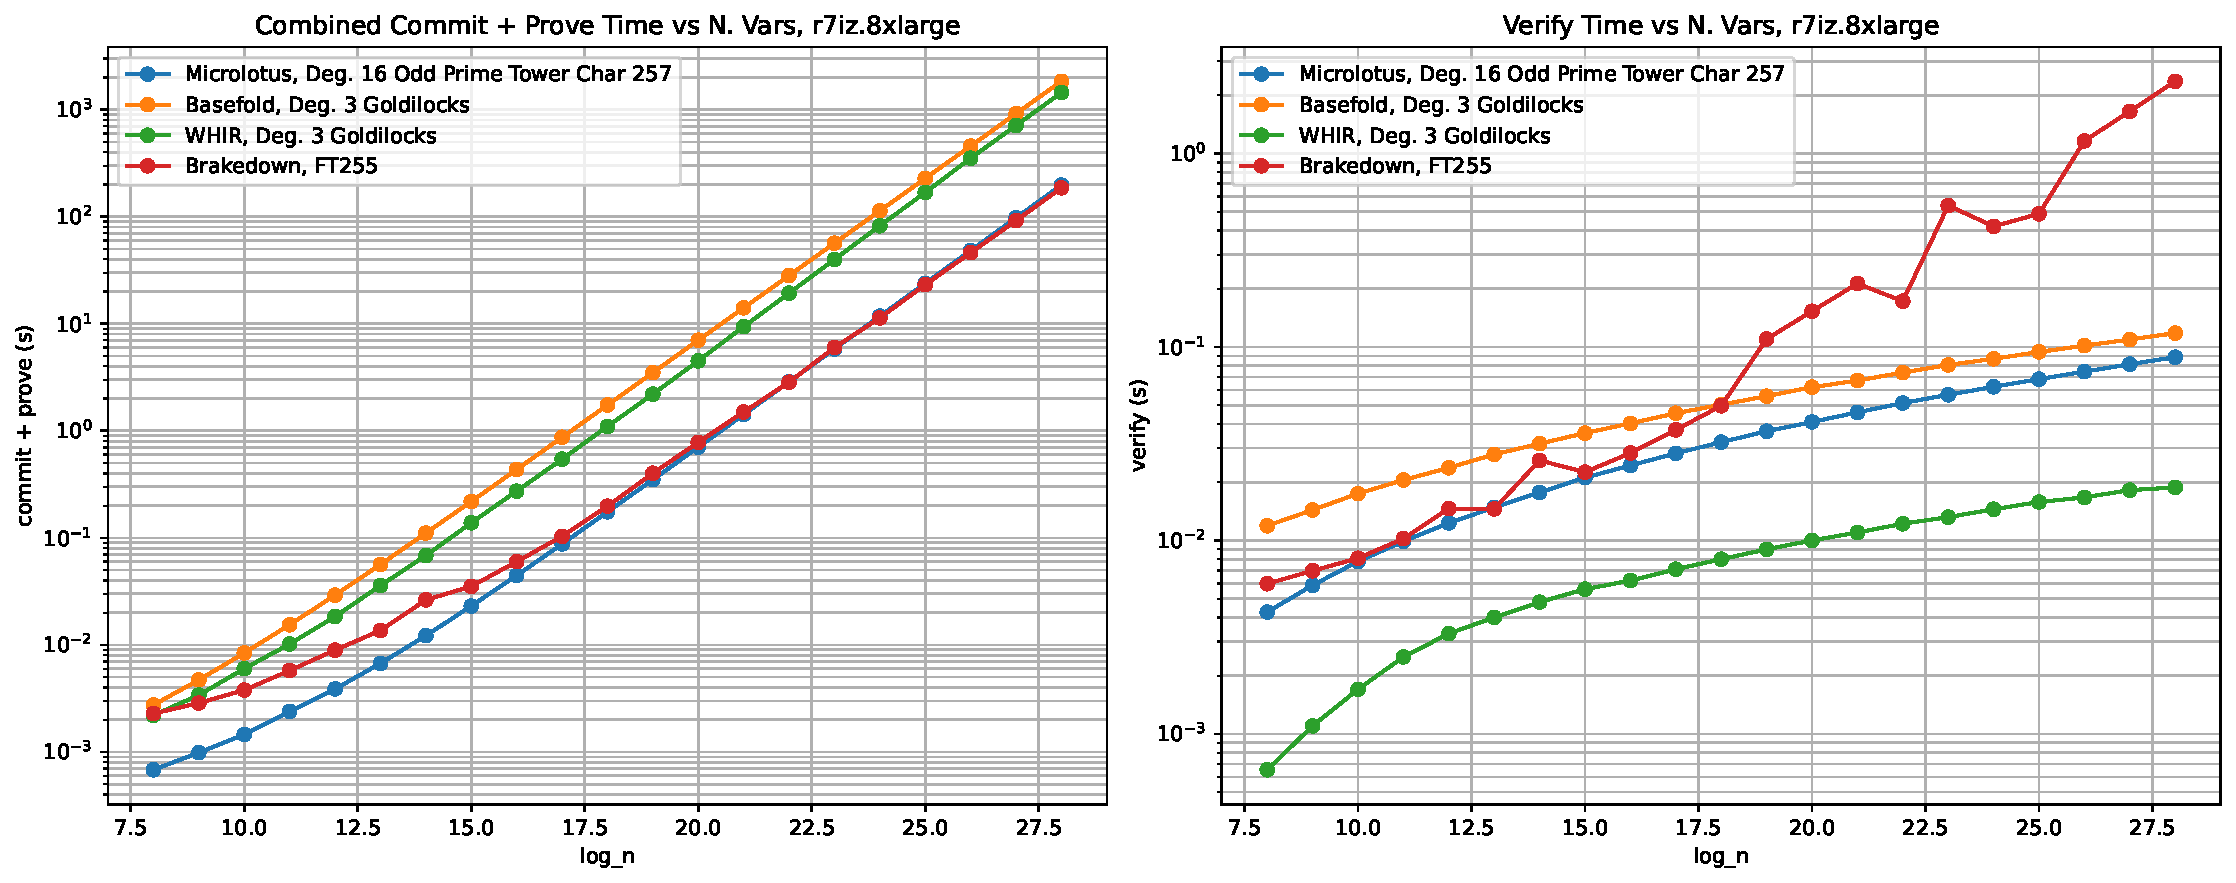
\includegraphics[width=\linewidth]{microlotus/plots/microlotus_odd_prime_tower_oracle_skip_1_folding_arity_1.pdf}
  \caption{Total Commit + Prove, Verify Times vs. $\log n$.}
\end{figure}

\begin{table}[h]

\centering
\renewcommand{\arraystretch}{0.6}
\setlength{\tabcolsep}{5pt}
\begin{tabular}{ l l l l l }
N. Vars & Commit + Prove & Verify & Proof Size \\
\hline
16 & 44.5ms & 24.4ms & 259.0 KiB \\
20 & 703.9ms & 41.0ms & 542.0 KiB \\
24 & 11.8s & 62.3ms & 931.2 KiB \\
28 & 197.4s & 88.6ms & 1430.8 KiB \\
\end{tabular}
\captionsetup{skip=5pt}
\caption{Microlotus PCS, Odd Prime Tower}

\centering
\renewcommand{\arraystretch}{0.6}
\setlength{\tabcolsep}{5pt}
\begin{tabular}{ l l l l }
N. Vars & Commit + Prove & Verify & Proof Size \\
\hline
16 & 434.9ms & 40.3ms & 568.2 KiB \\
20 & 7.0s & 62.0ms & 973.1 KiB \\
24 & 113.5s & 86.9ms & 1482.4 KiB \\
28 & 1840.5s & 117.9ms & 2114.8 KiB \\
\end{tabular}
\captionsetup{skip=5pt}
\caption{Basefold, Deg. 3 Goldilocks}

% \centering
% \renewcommand{\arraystretch}{0.6}
% \setlength{\tabcolsep}{9pt}
% \begin{tabular}{ l l l l }
% N. Vars & Commit + Prove & Verify & Proof Size \\
% \hline
% 16 & 585.6ms & 40.8ms & 544.0 KiB \\
% 20 & 9.8s & 61.7ms & 937.9 KiB \\
% 24 & 166.0s & 87.7ms & 1420.8 KiB \\
% 28 & 2796.6s & 117.8ms & 2038.4 KiB \\
% \end{tabular}
% \captionsetup{skip=5pt}
% \caption{Basefold, Odd Prime Tower}

\centering
\renewcommand{\arraystretch}{0.6}
\setlength{\tabcolsep}{5pt}
\begin{tabular}{ l l l l }
N. Vars & Commit + Prove & Verify & Proof Size \\
\hline
16  & 273.1 ms & 6.2 ms  & 287.5 KiB \\
20  & 4.5 s    & 10.0 ms & 413.3 KiB \\
24  & 82.3 s   & 14.5 ms & 558.8 KiB \\
28  & 1444.8 s & 18.8 ms & 712.8 KiB \\
\end{tabular}
\captionsetup{skip=5pt}
\caption{WHIR, Deg. 3 Goldilocks}

\centering
\renewcommand{\arraystretch}{0.6}
\setlength{\tabcolsep}{5pt}
\begin{tabular}{ l l l l }
N. Vars & Commit + Prove & Verify & Proof Size  \\
\hline
16 & 59.9 ms & 28.3 ms & 4.04 MiB  \\
20 & 780.1 ms & 153.0 ms & 9.11 MiB \\
24 & 11.3 s & 420.3 ms & 19.3 MiB \\
28 & 186.1 s & 2.4 s & 41.7 MiB \\
\end{tabular}
\captionsetup{skip=5pt}
\caption{Brakedown, Ft255}

\end{table}